\section{Admin Presentation} 

	\subsection{Requirements}
	
		\begin{enumerate}[itemsep=1pt,parsep=1pt]
			\item Creating organisational units.
			\item Move objects in the organisational hierarchy.
			\item Hierarchy of organisational units.
			\item Modify policies.
			\item Rules creation results in DSL script.
			\item Provide means of importing rules.
			\item Push updates to the client.
		\end{enumerate}
		
	\subsection{Technologies}
			
		\begin{itemize}
			\item \textbf{C\#} 
				\newline
				C\# is a multi-paradigm programming language encompassing strong typing, imperative, 
				declarative, functional, generic, object-oriented, and component-oriented programming disciplines. [cit]
		
			\item \textbf{AvalonDock} 
				\newline				
				Avalondock is a windows presentation foundation(WPF) controls library that provides the 
				functionality of a dockable layout system for UserControls within a user interface.  It supports fly-out panes
				dockable pinning expanders and floating windows.				
		
			\item \textbf{AvalonEdit} 
				\newline						
				Avalonedit is the WPF rich text user control for editing source code in SharpDevelop the open source 
				alternative to Visual Studio.  The editor features many of the post Intellij integrated development environment features
				such as code completion, code folding and syntax highlighting.
				
			\item \textbf{Infralution localization} 
				\newline						
				Infralution localization is an open source class library that integrates localisation features easily into
				windows presentation foundation(WPF) projects by taking control of resources files associated with a visual studio project.  
				This middle tier layer between the compiled code and the translations provides a means to instantly change
				the language in an application at run time.
				
			\item \textbf{JSON.net}	
				\newline								
				Json.Net is an open source Javascript Object Notation framework for .Net.  
				For message passing in the implementation between the nodes this was the preferably choice for message passing.
				
			\item \textbf{Microsoft Prism Event Aggregator}	
				\newline								
				The Microsoft implementation of Marting Fowler's Event Aggregator was chosen as a means for internal message
				passing within the application framework as it allows for events to be decoupled for the publishers and subscribers.
				
			\item \textbf{Visual Studio 2010}		
				\newline							
				The Microsoft Visual Studio Integrated Development Environment is by far the best in the field for rapid application 
				development in my opinion.  The deployment options, such as Web/Desktop/Phone etc
				coupled with the Common Language Runtime (CLR) run time environment allows for the development of applications that bring interoperability and manageability
				to new heights.
				
			\item \textbf{Windows Presentation Foundation}	
				\newline								
				The Windows Presentation Foundation graphical subsystem introduced with .Net 3.0 and at the core of Windows Vista / 7 
				renders applications directly into DirectX and is graphically accelerated on industry standard graphics cards.  The 
				idea of desktop compositioning driven by earlier projects in the open source community such as Beryl and Compiz
				made the push for this.  Apple and Microsoft quickly followed suit.  Furthermore WPF provides a model view-view model 
				design approach for the separation of the code and interface design somewhat comparable to Model View Controller introduced
				by smalltalk.
				
			\item \textbf{Xaml}		
				\newline							
				The Extensible Application Markup Language (Xaml) is a declarative XML based language used for the creation of user interfaces.
				Xaml directly maps for CLR run time object instances and the attributes to the associated properties allowing for most of the
				user interface functionally to be kept out of the business model or controller.
				
		\end{itemize}			
		
	\subsection{Design}
	
		\normalsize
		{	
			The design of the Linux Group Policy presentation or administrator interface was extensive.  With up wards of fifty 
			thousand lines of code, the need for a high quality design was exigent.  The support for the 'ilities' or non functional requirements
			motivated the design and eventual architectural framework.   Many influences lead to the design of the composite framework, such authors 
			as Martin Fowler, Joshua Kerievsky and Gamma et al.
			\newline	
			\newline
			Fig. \ref{fig:designoverview} presents a high level architectural design model.
			The design could be described as a three tier architecture.  Where the separation of presentation, logic and the data is shown.
			This distinction however in reality a little clouded, but the three tier architecture seems the best method to articulate the real nature
			of the design.	
			\newline
			\newline			
		}

		\begin{figurehere}
			\begin{center}
			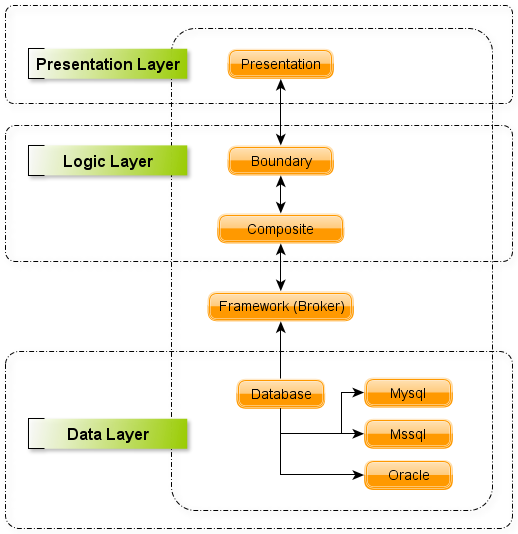
\includegraphics[scale=0.6]{pages/chapter3/figures/designarch.png}
			\end{center}
			\caption{Design Overview}
			\label{fig:designoverview}
		\end{figurehere}			

		\vspace{5mm}
		\normalsize
		{			
			Each composite has it's own responsibilities and encapsulates all the presentation and logic layers 
			for which it is concerned.  There are two composites that deviate from this assertion.
			\newline
			\newline
			It was decided upon to separate the data tier from the end composite developers.
			This separation of the data layer negates or reduces unfavourable database operations.
			The obfuscation of the structured query language(SQL) and the encapsulating of it into representing domain types provides traceability,
			monitoring and maintainability.
			\newline
			\newline
			The database composite is primarily concerned with the data layer, however it exhibits presentation (settings panes)
			and logic layer functionality also.  The database composite therefore abstracts all the domain concerns and the framework or the brokering layer 
			facilitates the access to this data layer or the database composite.
			\newline
			\newline
			The factory composite provides all the domain and architectural interfaces for the entire architecture.
			This framework layer decouples all composites and implements patterns to facilitate communication between these decoupled composites. 
			It does not provide a presentation or data layer, however it provides extensive logic layer functionality for the loading of the composites
			and subsequent brokered interactions.	
		}
		
\newpage
	
	\subsection{Architecture}		
				
		\vspace{-5mm}
		\begin{multicols}{2}
		
			The Architecture of the Linux Group Policy Studio Administration interface is comprised of separate interchangeable dynamic link libraries 
			as can be seen in the composite architectural overview in Fig. \ref{fig:archover}.  			
			This type of software technique is commonly known as composite or modular programming.  
			\newline
			\newline
			Each individual DLL (dynamic link library) is designed 
			for a specific scenario and encapsulates all the necessary logic for the scenario and its use cases.   
			This separation of concerns greatly improves the maintainability, reliability and reduces the fallibility of the software product as a whole.
			\newline
			\newline
			These dynamic link library components are loaded at run time and inspected via reflection for predefined architectural 
			interfaces.  Based on the interface the incorporation into the system is decided upon.  
			For example, if a class realises the interface IDatabaseStrategy,  we know this component is to be used by the Database connector 
			and therefore it is loaded and referenced in the appropriate location, making it accessible to the database connector.
			\newline
			\newline
			The main core of the modular framework consists of the lgp.components.factory dynamic link library which exposes the public static class 'Framework'.
			A static class is a class where all properties and methods are said to be static. C\# allows the use of the static keyword in the class definition
			thereby enforcing this rule. 
			\newline
			\newline
			Framework is a boundary class and with the use of the architectural and domain interfaces, it exposes the 
			dynamic link libraries concrete types that match, support, realise these interfaces.
			For example, rather that exposing the concrete Type 'Utilities' which is part of the framework;
			rather the interface for this type is exposed.  
		
			\columnbreak
		
			\begin{figurehere}
				\centering
				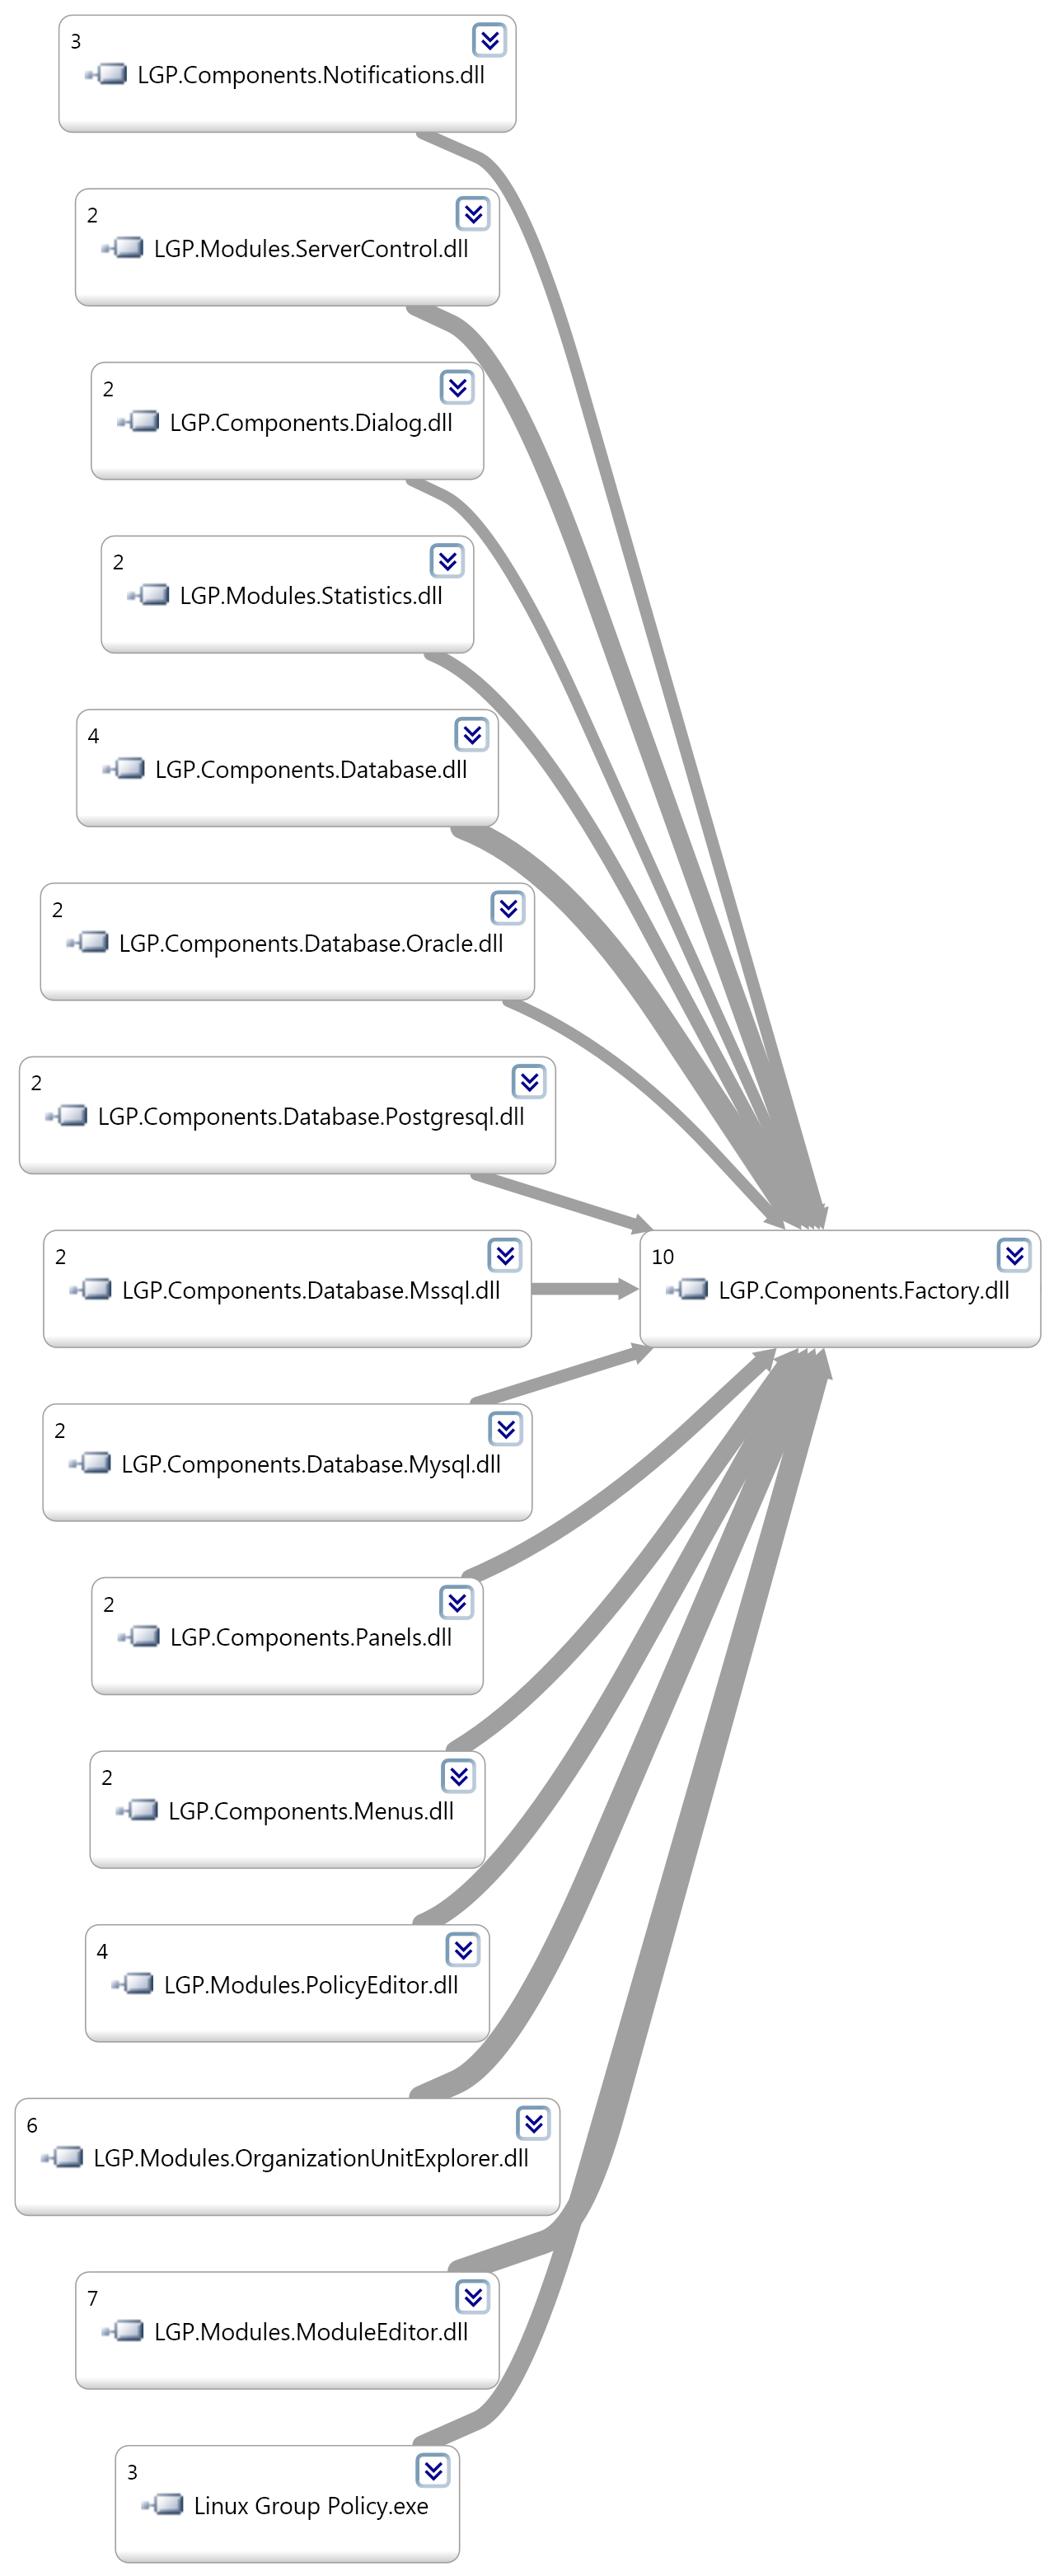
\includegraphics[scale=0.25]{pages/chapter3/figures/archover.png}
				\vspace{-2mm}
				\caption{Composite Architecture Overview}
				\label{fig:archover}
			\end{figurehere}	
		
		\end{multicols}
		
\newpage
				
		\normalsize
		{			
			This reduces the coupling and in effect the modules are not dependent on any one particular 
			concrete type other than that of the Framework boundary class.  The framework class exposes either directly or indirectly 38 separate interfaces 
			consisting of domain specific and non domain specific interfaces.  
			An excerpt of the framework class's auto properties (gets/sets) can be seen in Fig. \ref{fig:FrameworkClass}
			\newline
		}
		
		\indent\begin{minipage}{\textwidth}
			
			\begin{center}
			\begin{figurehere}
				\centering
				\inputminted[linenos=true,fontsize=\footnotesize,tabsize=2]{csharp}{pages/chapter3/smippets/framework.cs}
				\vspace{-5mm}
				\caption{Framework Static Class}
				\label{fig:FrameworkClass}
			\end{figurehere}	
			\end{center}
		
		\end{minipage}
			
		\vspace{5mm}	
		\normalsize
		{
			Where certain modular interaction is required the framework also provides a global uniform support for message passing.  This implementation 
			is based upon Martin Fowler's Event Aggregator design pattern.  This pattern allows publishers and subscribers to evolve independently of one 
			another, furthermore this modular approach to message passing fits well with the overall architectural design.  
			The published events of the event aggregator in the implementation are somewhat generic and therefore limited in application. 
			\newline
			\newline
			For specific interaction, an alternative approach was needed and the identification certain state transitions were identified 
			for exposure within the dynamic link library entity classes.  
			For example, right click context menus in modular systems are populated not only with menu options 
			from the implementing dynamic link library control class, but also the allowance or ability for other dynamic link library classes 
			to inject options into that menu as required.  
			\newline
			\newline
			This menu is generally specific to a type, ie. menu options for inode control 
			(file, directories) would not be applicable to a text editors right click menu.  Therefore differentiation of the specific 
			contexts are needed and in the framework implementation; these contexts are identified by the 38 separate interfaces Fig. \ref{fig:archinterfaces},
			specifically the domain specific interfaces Fig. \ref{fig:domaininterfaces}.  
			For third party developers, it is their choice whether or not to expose these transition states.
		}

		\vspace{3mm}
		\noindent\begin{minipage}{\textwidth}
			
			\begin{figurehere}
				\centering
				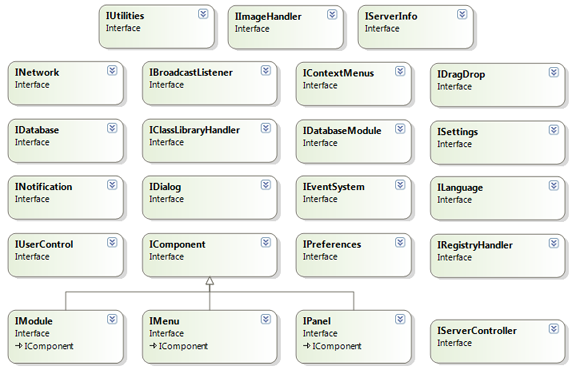
\includegraphics[scale=0.85]{pages/chapter3/figures/factory-interfaces-med.png}
				\caption{Architectural Interfaces}
				\label{fig:archinterfaces}
			\end{figurehere}
		
		\end{minipage}
		
		\vspace{3mm}
		\normalsize
		{
			An example of this within the application can be observed within the Organisational Unit explorer.  The right click menus on an Organisational
			Unit are exposed and the policy editor which is a separate independent module, injects its' ``edit policy'' menu.  The Event Aggregator pattern
			and Context Menu Injection Pattern can be referenced in section \ref{sec:LGPAdminCoding}.
			\newline
		}
							
		\large{\bfseries{Interfaces}}
		\newline		
		\normalsize
		{
			The architectural interfaces in Fig. \ref{fig:archinterfaces} \& \ref{fig:domaininterfaces} are used to decouple the dynamic link libraries from one another.
			These architectural interfaces are focused primarily with the inner workings of the application, the identification of 
			non domains specific classes, such as boundary or control classes concerned with user interface components, database access and networking.  
			\newline
			\newline			
			The following,  IOu, IClient, IGrammer, IPolicy and IModule are the domain specific interfaces.  The gateway interfaces are oriented around the
			Martin Fowlers' Table Gateway Pattern discussed later in this section, the subsequent observers and the separation of these interfaces.			
		}
			
		\noindent\begin{minipage}{\textwidth}
			
			\begin{figurehere}
				\centering
				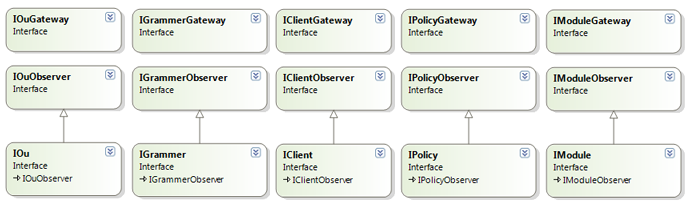
\includegraphics[scale=0.65]{pages/chapter3/figures/domainspecificinterfaces.png}
				\caption{Domain Specific Interfaces}
				\label{fig:domaininterfaces}
			\end{figurehere}
		
		\end{minipage}		
	
	\subsection{Patterns}
	
		\normalsize
		{	
			A key concern of any database centric product is the validity of the data.
			Dirty data in a database can lead to problems, for migrations and upgrades.  Research into the area revealed that many approaches to 
			controlling database access have been maturely established.  Many patterns were considered before implementation occurred. 
			Some of the design patterns considered where Query Object, Record Set, Row Data Gateway, Single Table Inheritance, Table Data Gateway, Table Module,
			Gateway, Active Record, Association Table mapping, Class Table Inheritance, Concrete Table Inheritance, Data Mapper and Data Session State to name a few.
			After careful consideration of uses cases, a modification of Table Data Gateway and Row Data Gateway was chosen. 
			\newline
		}
		
		\large{\bfseries{Table Data Gateway}}	
		\newline		
		\normalsize
		{			
			Table Data Gateway was an obvious candidate for manipulating a database table as a whole, from Patterns of Enterprise Application Architecture,
			Martin Fowler describes it as \emph{ "An object that acts as a gateway to a database table. One instance handles all rows in the table"  }	
			- \citet{FowlerPatternsArchiteture}. Simply put the Table Data Gateway is more like a collection data structure (list, arraylist, linkedlist), 
			smarts bits can be implemented to control or buffer the data too and from the database.
			\newline
			\newline
			This gateway implements methods similar to that found in the aforementioned collection types.  For example an Employee gateway
			would implement methods such as, get, add, remove and search.  These methods encapsulate the SQL ( structured query language ) statements
			that are used to query the database.  This abstracts database interaction from the plugin developers and reduces / negates the possibility of
			poorly constructed queries that may cause inefficient queries or in some cases harmful queries.  The following sample is used in the implementation
			as a control class for accessing the organisational unit table.
		}
			
		\vspace{2mm}
		\begin{figurehere}
			\inputminted[linenos=true,fontsize=\footnotesize,tabsize=2]{csharp}{pages/chapter3/smippets/ougateway}
			\vspace{-2mm}
			\caption{Organisational Unit Table Gateway}
			\label{fig:ougateway}
		\end{figurehere}

\newpage		
		
		\large{\bfseries{Row Data Gateway}}
		\newline
		\normalsize
		{
			\label{sec:RowDataGateway}
			On inspection of the interface in Fig. \ref{fig:ougateway} another type is recognised, ``Iou''.  This brings us to the second pattern Row Data Gateway
			and from Patterns of Enterprise Application Architecture, Martin Fowler describes it as \emph{ 
			"An object that acts as a gateway to a single record in a data source. There is one instance per row" } - \citet{FowlerPatternsArchiteture}.  
			As previously stated the Table Gateway can be described as a collection class and as a result Row Data Gateway complements this pattern.  
			\newline
			\newline
			Each row in the table is to be represented as an object in the system, to be encapsulated by the collection class.  
			Each column field within that row is a property of this object which needs to be encapsulated and appropriate rules or business logic embedded
			into accessors and mutators of this object.  This adds a second layer of data checking and enforcement of constraints to the data.  This second layer
			of perplexity ensures the reduction of dirty data in the tables. A database generally achieves this via foreign key constraints within the database.  
			However for fields in the database where constraints cannot be determined or accurately implemented via the internal data restriction mechanisms,
			the mutators of the object representation offer an area to ensure the validity of the data before updating the database.	
		}
		
		\vspace{5mm}
		\begin{figurehere}
			\inputminted[linenos=true,fontsize=\footnotesize,tabsize=2]{csharp}{pages/chapter3/smippets/ou}
			\vspace{-2mm}
			\caption{Organisational Unit Row Gateway}
			\label{fig:ou}
		\end{figurehere}
					
		\vspace{5mm}
		\normalsize
		{
			These two patterns in conjunction have many implementation concerns, such as the where and how updates are done.
			In this proof of concept implementation i decided to reduce the complexity and separate the concerns.  As such the 
			Table Gateway is concerned with managing the collection, and the row gateway is concerned with modifying its represented row.
			\newline
			\newline
			Developers may choose to use generics; also know as templates in C++, to implement generic gateways to be instantiated
			with specific types at run time.  This is an implementation concern that serves promote the re-usability of these gateways, however
			at the possible cost of security and control of the data, it was not decided to go this direction.
			\newline
		}	
		
\newpage
	
		\large{\bfseries{Event Aggregator}}
		
		\normalsize
		{
			The Event Aggregator design pattern by Martin Fowler is a publish subscribe design pattern.  Events are published 
			and subscribed to by means of an event handler control class.  This control class provides access to concrete implementations
			of composite presentation events which acts a broker for type based messages.
			\newline
			\newline
			Typical implementations of this pattern approach it in this manner, for the separation of event types.  
			The reason for this approach is that in large systems with many publishers and subscribers, the iteration of all the subscribers 
			for a published message, can be expensive.  Therefore the separation of the events and their composition event control classes is preferred.
			Fig. \ref{fig:EventAggregatorTypeBased} shows a high level overview of this approach.
			\newline
		}
		
		\begin{figurehere}
			\centering
			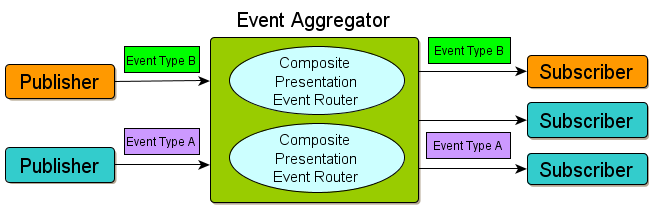
\includegraphics[scale=0.68]{pages/chapter3/figures/ean.png}
			\caption{Event Aggregator - type based}
			\label{fig:EventAggregatorTypeBased}
		\end{figurehere}
		
		\vspace{5mm}
		\normalsize
		{
			For a large architecture, this is the ideal approach for the best performance, security and decoupling concerns.
			However in the project these concerns did not out way the overhead of the separation of events, their handlers, their interfaces
			and the overall increase of types and resulting coupling within the system.  Therefore I decided to use a generics approach.
			By creating a generic composite presentation event router and with the use of domain interfaces this explosion of types
			was negated.  I left it up to the subscriber to determine whether the message that was received was of the type it was concerned with.
			This moved the responsibility of the type interpretation from the event router to the event receiver.	Fig. \label{fig:EventAggregatorGenericBased}
			presents this generics approach.
			\newline
		}
		
		\begin{figurehere}
			\centering
			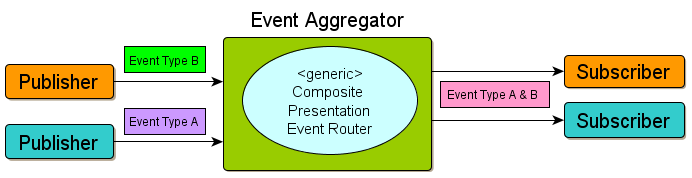
\includegraphics[scale=0.62]{pages/chapter3/figures/eag.png}
			\caption{Event Aggregator - generic based}
			\label{fig:EventAggregatorGenericBased}
		\end{figurehere}
		
\newpage
	
	\subsection{Coding} 
		\label{sec:LGPAdminCoding}
			
			
		\normalsize
		{		
			Unlike the relatively simplistic flexibility of interpreted languages, the implementation of the presentation user interface required
			greater knowledge.  A deep understanding of the concepts of binding, dynamic dispatch and reflection had to be well understood in order
			to create the composite architecture.
			The knowledge base required was not limited to these fundamental or computer science software characteristics.
			An understanding of user interface design and concepts such as routed events and event bubbling was mandatory.
			\newline
			\newline
			In this section i will attempt to articulate these concepts, as they were used in the software architecture developed.
			\newline
		}
		
		\large{\bfseries{Reflection and the loading of composites}}
		\newline
		\normalsize
		{
			As previously discussed in the architectural overview, the composite approach is achieved via the use of reflection.  
			Reflection is a process by which a computer program can inspect a type at run time.  It is not limited to just inspection,
			as it can be used to modify an objects structure and behavior at run time.  In the architectural design however, reflection is 
			primarily used for inspection of the of composites and their internal types.  These types that match, support, realise architectural interfaces
			are loaded and referenced in the appropriate location.  These objects are then exposed via the Framework static class as previously discussed.
			\newline
			\newline
			Fig. \ref{fig:reflection} presents an example of the use of reflection.  In this example a composite or assembly is loaded and
			through this assembly reference, the inspection of it's internal types is done.
			The goal in this example, is the search for a type that realises the IContextMenus interface.  When it is found, it is assigned to 
			an internal member property, which can then be later accessed via an accessor (GET method).
			\newline
		}
		
		\begin{figurehere}
			\inputminted[linenos=true,fontsize=\footnotesize,tabsize=2]{csharp}{pages/chapter3/smippets/reflection}
			\caption{Using reflection to load modules}
			\label{fig:reflection}
		\end{figurehere}
		
		
		
		
		\large{\bfseries{Exposing of these loaded types}}
		\newline
		\normalsize
		{
			As seen here in Fig. \ref{fig:reflection} which is an excerpt of the ClassLibraryHandler class, a class that realises
			this IContextMenus is loaded and exposed.  To put this in context, Fig. \ref{fig:framework} shows the exposure of this 
			type via the Framework static class.  The type exposed is the interface and not the concrete type, therefore this effectively decouples 
			other composites from the concrete implementation of said type.  In order to make use of this functionality, other composites
			include a reference to the Framework static class.
		}

		\vspace{5mm}
		\begin{figurehere}
			\inputminted[linenos=true,fontsize=\footnotesize,tabsize=2]{csharp}{pages/chapter3/smippets/framework}
			\vspace{-5mm}
			\caption{Framework exposing plug-ins via interfaces}
			\label{fig:framework}
		\end{figurehere}
		
		
		
		
		
				
		\vspace{3mm}
		\large{\bfseries{IContextMenus}}
		\newline
		\normalsize
		{	
			Following on from the loading and exposing of this type, Fig. \ref{fig:IContextMenusinterface} depicts the method signatures of this interface.
			This interface provides access to the architectural support, for registering of menu items, in context menus dynamically at run time.  
		}
				
		\vspace{4mm}
		\begin{figurehere}
			\inputminted[linenos=true,fontsize=\footnotesize,tabsize=2]{csharp}{pages/chapter3/smippets/IContextMenus.cs}
			\vspace{-5mm}
			\caption{IContextMenus interface}
			\label{fig:IContextMenusinterface}
		\end{figurehere}
		
		
		
		
		
		
		\vspace{3mm}
		\normalsize
		{		
			The RegisterContextMenuItem allows plug-ins to register menu items to be dynamically embedded into a context menu.  The three parameters 
			specify the type that will be passed back to the registering handler, the menu item which will physically be displayed in the context menu and 
			finally the Action, which is a delegate for an encapsulated callback method.
			\newline
			\newline
			In Figure \ref{fig:registration} plugin A registers menu items with the context menus handler (IContextMenus).
			The callback method, the final destination of the menu item click is where the ITargetItem is sent. 
			\newline
		}
			
		\vspace{-2mm}
		\begin{figurehere}
			\inputminted[linenos=true,fontsize=\footnotesize,tabsize=2]{csharp }{pages/chapter3/smippets/registerMenuItem}
			\caption{Plugin A : Register menu item with the framework}
			\label{fig:registration}
		\end{figurehere}
			
		\vspace{3mm}
		\normalsize
		{
			In Figure \ref{fig:attachregistration} plugin B accepts menu registrations for ItargetType and requests the 
			context menus handler (IContextMenus) to append them to the context menu. The menu item click handles the actual click event.
			This allows ``smart bits'' to occur before asking the context menus handler (IContextMenus) to invoke the CallBackMethod in plugin A.
			This decouples the plug-ins from one another, coupling the two with IContextMenus and any ``Type'' in this instance ITargetType.
			\newline
		}	
					
			
		\begin{figurehere}
			\inputminted[linenos=true,fontsize=\footnotesize,tabsize=2]{csharp}{pages/chapter3/smippets/contextOpeningEvent}
			\vspace{-2mm}
			\caption{Plugin B : Handle menu item click and invoke callback}
			\label{fig:attachregistration}
		\end{figurehere}			
			

		
		

		\vspace{3mm}
		\large{\bfseries{Dynamic Context Menus Sequence Diagram}}
		\newline
		
		\begin{figurehere}
			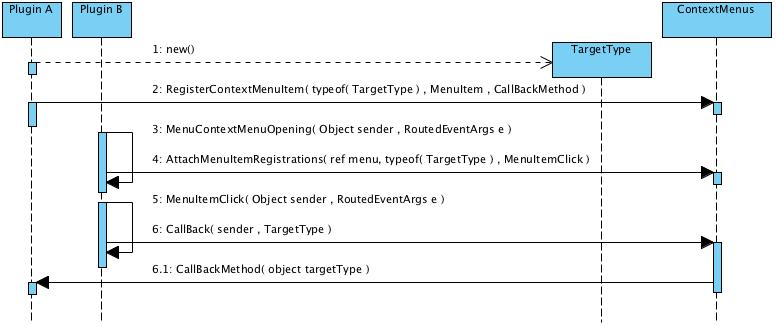
\includegraphics[scale=0.6]{pages/chapter3/figures/SequenceContextMenus2.jpg}
			\caption{Context Menus hooks sequence diagram}
		\end{figurehere}
						

\newpage
						

	\subsection{Analysis}
	
		\normalsize
		{	
			A widely accepted concept in software design is the decoupling of components(composites) or the minimisation of inter dependencies, to promote re-usability.  
			There are many papers that target interface definition as the means to accomplish this, such as, 
			``A comprehensive interface definition framework for software components'' \& ``An Approach to Software Component Specification'' by \citet{JunHan}.
			With this software paradigm preposition, I am going take a look at the more fundamental concern of component (composite) based design. 
			\newline
			\newline
			David Lloyd of JGroup Expert defines the distinction between libraries and frameworks :
		}	
			
		\vspace{-5mm}
		\begin{multicols}{2}
		
			\begin{itemize}		
				
				\item \textit{\textbf{Library}}	
				
					\begin{itemize}
			
						\item \textit{Set of classes instantiated by client}							
						\item \textit{Client calls functions}		
						\item \textit{No predefined flow of control}
						\item \textit{No predefined interaction}
						\item \textit{No default behaviour}						
					
					\end{itemize}
				

		\columnbreak
					
				\item \textit{\textbf{Framework}}	

					\begin{itemize}
			
						\item \textit{Customisation by sub-classing}							
						\item \textit{Calls client functions}	
						\item \textit{Controls flow of execution}							
						\item \textit{Defines object interaction}	
						\item \textit{Provides default behaviour}	
					
					\end{itemize}
					
			\end{itemize}

		\end{multicols}
		
		\vspace{-2mm}
		\normalsize
		{		
			Given the aforementioned premises of architectural design goals and the distinction between libraries and frameworks; 
			it may seem that libraries do not exhibit characteristics prevalent to achieve decoupled components (composites).  The instantiation
			of classes and calling of functions directly, couples components (composites).
			\newline
			\newline		
			Composite design therefore even with good interfaces and supporting factory methods still presents coupling.  This coupling as stated comes in the form 
			of factory methods that require access to one or more concrete types in a composite.  If there are multiple interdependencies between composites
			changing out a composite may present difficultly in the form of refactoring.
			\newline
			\newline
			The fundamental concern is then composite interdependencies.  The characteristics of a framework provide greater composite decoupling.  
			The presentation framework for the admin interface provides only one concrete dependency relationship, targeting this concern.		
			The admin presentation interface evolved to the characteristics of a framework, which I believe is a bigger concern, than good interface
			definition.  This concept comparable to networking is the difference between a mesh network and a star network, as seen in Fig. \ref{fig:Interdependance}.
			\newline
		}
		
		\begin{figurehere}
			\centering
			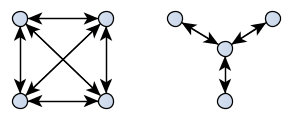
\includegraphics[scale=1.0]{pages/chapter3/figures/interdependance.png}
			\caption{Interdependence - Mesh(L) - Star(R)}
			\label{fig:Interdependance}
		\end{figurehere}
	
\newpage	
	
	\subsection{Improvements}

		There are many advantages and disadvantages to the framework developed.  The architectural framework devised is rigid in many respects.  
		As all classes in the factory composite are defined as ``internal'' classes and exposed via their interfaces, this does not offer any sub-classing 
		and changing of behaviour to composite developers.  This effectively locks developers into the behaviour of the architectural framework.
		\newline
		\newline
		To address this concern, firstly the reasoning for this approach must first be addressed.  During coding it is common practice to exercise encapsulation
		when implementing classes and through the use of accessors and mutators, this basic object oriented principle is adhered to.  Similarly when designing composites
		this practice can be achieved via ``internal'' classes.  This effectively means that peer composites cannot instantiate these classes marked as internal.
		\newline
		\newline
		For future improvements to the architectural framework, a relaxing of this principle may be applied.  Classes that are not deemed critical to core
		functionality or do not present a security concern, may be marked as public.  Alternatively patterns to support other functionality or
		out of band services would be the preferred approach.  An analysis of composite developer requirements should be completed and patterns implemented in 
		future revisions to support these requirements.
		
		
